\documentclass[conference]{IEEEtran}

\usepackage{cite}
\usepackage{amsmath,amssymb}
\usepackage{graphicx}
\usepackage{booktabs}
\usepackage{tikz}
\usepackage{xcolor}
\usepackage{hyperref}
\usepackage{pgfplots}
\usepackage{tabularx}
\usepackage{array}
\pgfplotsset{compat=newest}

\hypersetup{
    colorlinks=true,
    linkcolor=blue,
    citecolor=blue,
    urlcolor=blue
}

\newcolumntype{Y}{>{\raggedright\arraybackslash}X}

\begin{document}

\title{Historical Case Study on Ti Silicide (TiSi\textsubscript{2}) \\ Reliability Issues in Mixed-Voltage CMOS Driver ICs}

\author{
\IEEEauthorblockN{Shinichi Samizo}
\IEEEauthorblockA{Independent Semiconductor Researcher\\
Project Design Hub, Samizo-AITL\\
\textit{Email:} \href{mailto:shin3t72@gmail.com}{shin3t72@gmail.com}\quad
\textit{GitHub:} \href{https://github.com/Samizo-AITL}{Samizo-AITL}}
}

\maketitle

\begin{abstract}
This paper analyzes a historical failure case at the 0.25~µm CMOS node related to Ti silicide (TiSi\textsubscript{2}) phase-transition instability.
For active-matrix TFT (aTFT) LCD driver ICs that required mixed 3.3~V logic and $\sim$30~V high-voltage (HV) devices, manufacturers selected the 0.25~µm process because its LOCOS isolation safely supported HV co-integration.
By contrast, the 0.18~µm STI-based node, although denser and yield-stable, posed edge-thinning risks for $\sim$30~V devices and required a new HV platform.
Incomplete C49$\rightarrow$C54 transformation with boron absorption created localized high-resistance spots, directly reducing 1~Mbit SRAM yield.
The study highlights how process optimization and empirical feedback cycles were indispensable when isolation technology and device requirements constrained node selection.
\end{abstract}

\section{Introduction}
In the late 1990s, LCD driver ICs for passive monochrome panels were commonly fabricated in 0.35~µm processes supporting 3.3~V logic and 40~V HV devices.
With the transition to active-matrix TFT (aTFT) LCD panels in the early 2000s, driver ICs required higher-performance logic, embedded large SRAM macros, and continued HV integration around 30~V.

Although the 0.18~µm CMOS process was already in mass production with small die size and stable yield, it relied on Shallow Trench Isolation (STI), where edge thinning introduced a reliability risk for $\sim$30~V devices.
By contrast, the 0.25~µm process used Local Oxidation of Silicon (LOCOS), which had a proven track record for HV isolation.
Therefore, manufacturers adopted the 0.25~µm LOCOS-based process for 3.3~V + 30~V LCD driver ICs, accepting area disadvantages to guarantee HV compatibility.

\begin{table*}[!t]
\centering
\caption{Comparison of 0.25\,\textmu m LOCOS and 0.18\,\textmu m STI nodes for LCD driver ICs}
\label{tab:node_compare}
\setlength{\tabcolsep}{4pt}\footnotesize
\begin{tabularx}{\textwidth}{@{}lYY@{}}
\toprule
& \textbf{0.25\,\textmu m (LOCOS)} & \textbf{0.18\,\textmu m (STI)} \\
\midrule
Isolation method & Thick field oxide (LOCOS); proven HV margin & Shallow trench isolation; edge thinning risk at HV corners \\
HV device support (at that time) & Existing $\sim$30\,V HV design reusable & New HV platform required (re-qualification) \\
Die size / density & Larger die, lower density & Smaller die, higher density \\
Yield stability & Moderate; yield impacted by TiSi\textsubscript{2} instability & Stable baseline process with CoSi\textsubscript{2} salicide \\
Embedded SRAM redundancy & Not implemented (design/area/timing overhead); no laser repair in mixed-signal testers & Same limitation; redundancy/laser repair infeasible in LCD driver IC test flow \\
Risk at 1\,Mbit SRAM & High: localized resistive defects $\Rightarrow$ chip rejection & Lower base risk, but HV co-integration not yet qualified \\
Adoption rationale & Safe HV compatibility outweighed cost/density & Density/yield advantage offset by HV risk; not adopted for HV driver products \\
\bottomrule
\end{tabularx}
\end{table*}

\section{Technical Background}
\subsection{Isolation Choice for HV Devices}
\begin{itemize}
    \item \textbf{0.25~µm LOCOS:} Mature, thick field oxide with well-established margins for $\sim$30~V HV device integration.
    \item \textbf{0.18~µm STI:} Provided density and yield benefits, but corner thinning at the trench edge raised leakage and breakdown concerns for HV devices, necessitating a new HV device platform.
\end{itemize}

\subsection{Ti Silicide Phase Transformation in Detail}
TiSi\textsubscript{2} undergoes a polymorphic phase transition from
the metastable C49 phase (orthorhombic, resistivity $\sim$60--90~µ$\Omega\cdot$cm)
to the stable C54 phase (tetragonal, $\sim$15--20~µ$\Omega\cdot$cm).
This transformation is typically induced by RTA in the 650--750~°C range.
Incomplete transformation leaves residual C49 grains, which behave as
localized resistive defects.
Boron absorption from halo implants further aggravated resistivity variation,
narrowing the process window for stable transformation.

\subsection{Silicide Evolution at the 0.18~µm Node}
Another reason for higher baseline yield at the 0.18~µm node was the
industry-wide transition from TiSi\textsubscript{2} to CoSi\textsubscript{2}.
Unlike TiSi\textsubscript{2}, which required a C49$\rightarrow$C54 transformation,
CoSi\textsubscript{2} formed directly in the stable low-resistivity phase
($\sim$15--20~µ$\Omega\cdot$cm). This eliminated random resistive spots
from incomplete phase change, improved process windows, and enhanced
compatibility with scaled junctions. Although 0.18~µm STI was unsuitable
for HV integration at that time, its logic baseline process achieved
stable yield.

\section{Failure Analysis}
\subsection{Observation: 1~Mbit SRAM}
In mass production, random single-bit failures appeared in the 1~Mbit SRAM macro. Since redundancy was not implemented in the embedded macro, even a single defective bit caused rejection of the entire device.

\begin{figure}[!t]
  \centering
  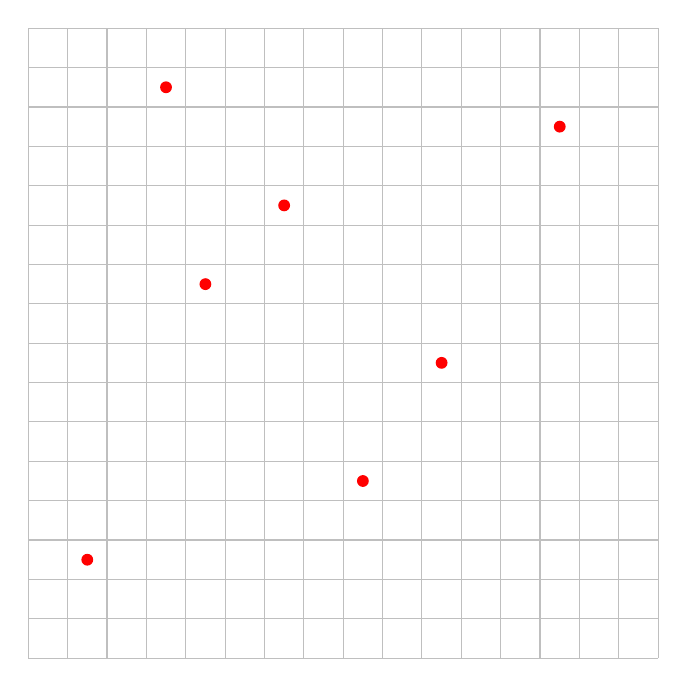
\begin{tikzpicture}[scale=0.5]
    \draw[step=1cm,gray!50,thin] (0,0) grid (16,16);
    % Defect points
    \foreach \x/\y in {2/3, 5/10, 7/12, 9/5, 11/8, 14/14, 4/15} {
      \fill[red] (\x-0.5,\y-0.5) circle (0.15);
    }
  \end{tikzpicture}
  \caption{Example of random single-bit failure map in a 1~Mbit SRAM. Red dots represent defective bits scattered randomly across the array.}
  \label{fig:failmap}
\end{figure}

\subsection{Redundancy Limitation in Embedded Macros}
In stand-alone memory products, redundancy circuits are standard practice and defective cells can be repaired during testing via laser trimming.
In embedded memory macros, however, redundancy is generally excluded due to design complexity, timing, and area overhead.
Additionally, LCD driver ICs were typically tested on mixed-signal/SoC testers, which lacked built-in support for redundancy repair.
Therefore, redundancy was not adopted, and scaling to 1~Mbit carried critical reliability risk.

\subsection{Root Cause}
Failure localization confirmed that:
\begin{itemize}
    \item Boron from halo regions diffused into Ti during silicidation.
    \item Local B uptake inhibited C54 transformation, leaving high-resistance C49 spots.
    \item These spots manifested as random SRAM bit failures.
\end{itemize}

\subsection{Review Limitation}
Earlier 500~kbit SRAM macro products had not shown this issue. Based on those precedents, engineers assumed that scaling to 1~Mbit would be safe.
Consequently, the failure mode was not identified during the initial development review stage, demonstrating the limitation of relying on past yield experience without revalidation.

\begin{table}[!t]
\centering
\caption{Estimated yield impact from scaling embedded SRAM capacity}
\label{tab:yield_scaling}
\setlength{\tabcolsep}{4pt}
\begin{tabular}{lcc}
\toprule
Macro Size & Observed Failures & Yield Estimate \\
\midrule
500 kbit & Rare, localized & $\sim$95\% \\
1 Mbit   & Frequent, random & $\sim$70\% \\
\bottomrule
\end{tabular}
\end{table}

\section{Countermeasures}
\subsection{Provisional Measures: Sidewall Deposition + Etch-Back (Foot Under-etch)}
A conformal dielectric (e.g., oxide or nitride) was deposited on the STI
sidewall and then anisotropically etched back, leaving a slight recess/foot
at the sidewall bottom. This \textbf{sidewall deposition + etch-back} flow
increased the lateral separation between the halo implant extension and the
silicide formation front at the active edge. As a result, boron encroachment
into Ti was suppressed and the \textbf{generation of residual C49 high-resistivity
grains was prevented}, stabilizing yield. Because the effect still relied on
tight process-window control (liner thickness, etch-back dose, corner profile),
lot-to-lot robustness was not guaranteed; therefore the measure was treated
as a provisional fix.

% ===== Fig.2: Cross-sections based on user's sketch =====
\begin{figure*}[!t]
  \centering
  \resizebox{\textwidth}{!}{%
  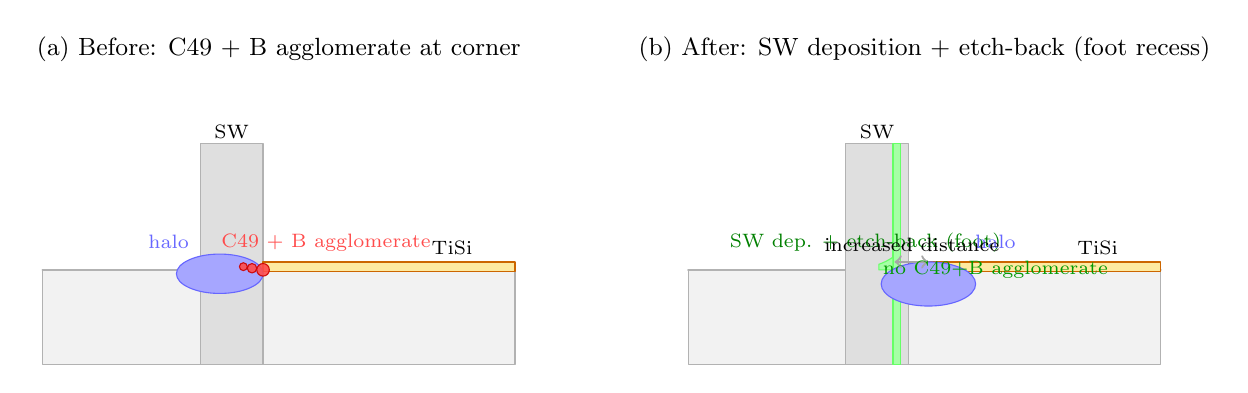
\begin{tikzpicture}[x=1cm,y=1cm,line cap=round,line join=round]
    % styles
    \tikzstyle{si}=[fill=gray!10,draw=gray!60]
    \tikzstyle{oxide}=[fill=gray!25,draw=gray!60]
    \tikzstyle{silicide}=[fill=yellow!60!orange!35,draw=orange!80!black]
    \tikzstyle{halo}=[fill=blue!35,draw=blue!60]
    \tikzstyle{spacer}=[fill=green!35,draw=green!60]
    \tikzstyle{label}=[font=\scriptsize]
    \tikzstyle{residual}=[fill=red!70,draw=red!80!black,opacity=0.9]

    % ----------------------------------------------------
    % (a) BEFORE : per sketch
    % ----------------------------------------------------
    \begin{scope}[shift={(0,0)}]
      \node[font=\small] at (3.0,2.8) {(a) Before: C49 + B agglomerate at corner};
      % silicon substrate (right side active)
      \path[si] (0,-1.2) rectangle (6,0);
      % surface line
      \draw[gray!60,thick] (0,0) -- (6,0);
      % sidewall (SW)
      \path[oxide] (2.0,-1.2) rectangle (2.8,1.6);
      \node[label] at (2.4,1.75) {SW};

      % TiSi (silicide) on surface (active to the right of SW)
      \path[silicide] (2.8,-0.02) rectangle (6,0.10);
      \node[label] at (5.2,0.28) {TiSi};

      % halo (touching the corner)
      \draw[halo] (2.25,-0.05) ellipse (0.55 and 0.25);
      \node[label,blue!60] at (1.6,0.35) {halo};

      % C49 + B agglomerate (at the corner)
      \draw[residual] (2.80,0.00) circle (0.08);
      \draw[residual] (2.66,0.02) circle (0.06);
      \draw[residual] (2.55,0.04) circle (0.05);
      \node[label,red!70] at (3.6,0.35) {C49 + B agglomerate};
    \end{scope}

    % ----------------------------------------------------
    % (b) AFTER : sidewall deposition + etch-back (foot recess)
    % ----------------------------------------------------
    \begin{scope}[shift={(8.2,0)}]
      \node[font=\small] at (3.0,2.8) {(b) After: SW deposition + etch-back (foot recess)};
      % silicon
      \path[si] (0,-1.2) rectangle (6,0);
      \draw[gray!60,thick] (0,0) -- (6,0);
      % sidewall body
      \path[oxide] (2.0,-1.2) rectangle (2.8,1.6);
      \node[label] at (2.4,1.75) {SW};

      % sidewall liner (deposition) and foot recess after etch-back
      \path[spacer] (2.70,-1.2) -- (2.60,-1.2) -- (2.60,1.6) -- (2.70,1.6) -- cycle; % liner
      % foot recess (small under at the foot)
      \fill[spacer] (2.60,0) -- (2.60,0.16)
         .. controls (2.54,0.12) and (2.48,0.09) .. (2.42,0.07)
         -- (2.42,0) -- cycle;
      \node[label,green!50!black] at (2.25,0.35) {SW dep. + etch-back (foot)};

      % TiSi (silicide) on surface
      \path[silicide] (2.8,-0.02) rectangle (6,0.10);
      \node[label] at (5.2,0.28) {TiSi};

      % halo (now separated from corner)
      \draw[halo] (3.05,-0.18) ellipse (0.60 and 0.28);
      \node[label,blue!60] at (3.9,0.35) {halo};

      % spacing arrow (lateral separation)
      \draw[<->,thick,gray!70] (2.62,0.10) -- (3.05,0.10);
      \node[label] at (2.84,0.32) {increased distance};

      % no residual marker
      \node[label,green!60!black] at (3.9,0.00) {no C49+B agglomerate};
    \end{scope}
  \end{tikzpicture}}
  \caption{Cross-sections near a sidewall (SW) following the user's sketch.
  (a) Before: the halo approaches the surface at the SW corner, forming a C49\,+\,B agglomerate that perturbs silicidation.
  (b) After: sidewall \emph{deposition} and anisotropic \emph{etch-back} create a liner and a slight foot recess, securing lateral distance between the halo extension and the TiSi front.}
  \label{fig:fig2_sw_sketch}
\end{figure*}

\subsection{Permanent Measures: Ramp Anneal Optimization}
Ramp-anneal conditions were optimized (ramp rate and soak time)
to \textbf{complete the C49$\rightarrow$C54 transformation}. This
stabilized silicide resistivity, but altered device characteristics
(e.g., series resistance, contact resistance, and junction leakage).
As a result, device models, RC extraction data, and timing libraries
required \textbf{re-characterization across PVT corners}. Thus, the
permanent solution involved a trade-off between silicide stability and
the cost of revalidating circuit-level parameters.

\section{Yield Sensitivity Model}
The yield impact of redundancy can be approximated by a Poisson model:
\[
Y_k = e^{-\lambda} \sum_{i=0}^{k} \frac{\lambda^i}{i!},
\]
where $\lambda$ is the average defect count and $k$ is the redundancy capacity.

\begin{figure}[!t]
  \centering
  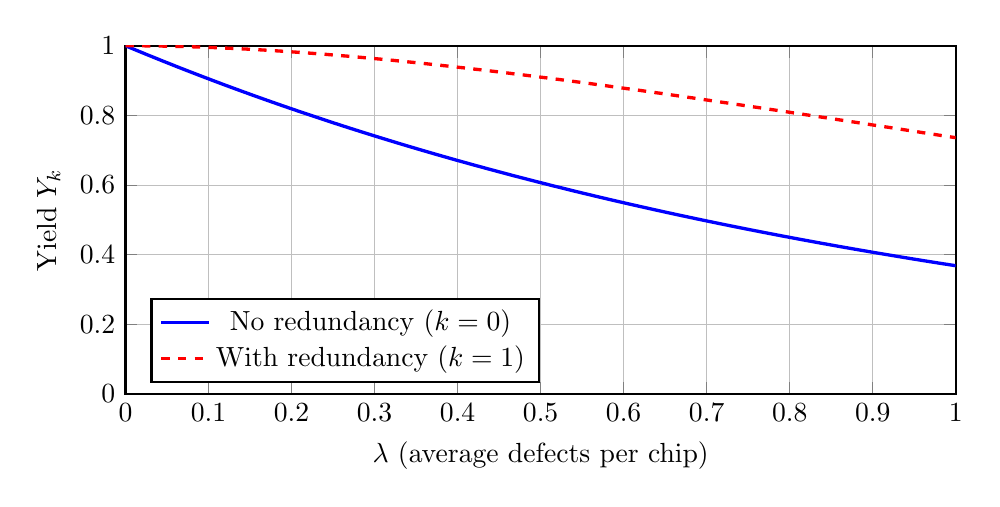
\begin{tikzpicture}
    \begin{axis}[
      width=\columnwidth,
      height=6cm,
      xlabel={$\lambda$ (average defects per chip)},
      ylabel={Yield $Y_k$},
      xmin=0, xmax=1,
      ymin=0, ymax=1,
      legend pos=south west,
      grid=both,
      major grid style={line width=.2pt,draw=gray!50},
      minor grid style={line width=.1pt,draw=gray!20},
      thick,
    ]
      \addplot[blue, very thick, domain=0:1, samples=200] {exp(-x)};
      \addlegendentry{No redundancy ($k=0$)}
      \addplot[red, dashed, very thick, domain=0:1, samples=200] {exp(-x)*(1+x)};
      \addlegendentry{With redundancy ($k=1$)}
    \end{axis}
  \end{tikzpicture}
  \caption{Illustrative yield sensitivity (Poisson model) with and without redundancy.}
  \label{fig:yield}
\end{figure}

\section{Educational Application}
\subsection{Teaching Tools}
\begin{itemize}
    \item Cause-effect diagrams: process $\rightarrow$ defect $\rightarrow$ yield
    \item Comparative analysis: 0.25~µm (LOCOS) vs 0.18~µm (STI) for HV devices (Table~\ref{tab:node_compare})
    \item Exercises: prioritize process fix vs. redundancy adoption
\end{itemize}

\subsection{Exercises}
\begin{enumerate}
  \item Using Eq.~(1), compute the yield for $\lambda=0.2$ and 0.5 with and without redundancy ($k=0,1$).
  \item Based on Table~\ref{tab:node_compare}, discuss which node (0.25~µm LOCOS or 0.18~µm STI) you would adopt if tasked with designing a 3.3~V + 30~V mixed-signal IC in 2000.
\end{enumerate}

\subsection{Lessons}
This case shows the risk of extrapolating from small macros (500~kbit) to larger ones (1~Mbit) without reassessing defect sensitivity.
It also emphasizes that process-related instability, invisible at smaller scales, can dominate yield once redundancy is unavailable.
For embedded SRAM, capacity scaling must always be coupled with explicit yield-risk validation.

\section{Conclusion}
This case demonstrates how HV compatibility constraints dominated node selection.
Despite the availability of a denser, yield-stable 0.18~µm STI process with CoSi\textsubscript{2} salicide, the requirement for safe $\sim$30~V HV integration drove adoption of 0.25~µm LOCOS.
Yield loss from incomplete TiSi\textsubscript{2} phase transformation (with boron absorption) became critical at the 1~Mbit SRAM scale.
The educational value lies in showing how scaling, process technology, and reliability intersect, and why continuous empirical feedback is essential.
Although the analysis here focused on SRAM macros, the same lesson applies to mixed-signal SoCs and aTFT driver ICs: process-induced variability, once coupled with system-level design constraints, can dominate yield and reliability.

\begin{thebibliography}{99}
\bibitem{Sze2007} S. M. Sze and K. K. Ng, \textit{Physics of Semiconductor Devices}, 3rd ed. Wiley, 2007.
\bibitem{Wolf1986} S. Wolf and R. N. Tauber, \textit{Silicon Processing for the VLSI Era, Vol. 1: Process Technology}. Lattice Press, 1986.
\bibitem{Colinge2004} J.-P. Colinge, \textit{Silicon-on-Insulator Technology: Materials to VLSI}, 3rd ed. Springer, 2004.
\bibitem{ITRS2001} International Technology Roadmap for Semiconductors (ITRS), ``Process Integration, Devices, and Structures,'' 2001.
\bibitem{Takeda1994} E. Takeda, C. Y. Yang, and A. S. Grove, ``Silicide technology for ULSI applications,'' \textit{IEEE Trans. Electron Devices}, vol. 41, no. 12, pp. 2133--2141, Dec. 1994.
\bibitem{Chang1996} J. P. Chang and A. J. Steckl, ``Titanium silicide formation and stability in submicron CMOS technology,'' \textit{J. Appl. Phys.}, vol. 79, no. 9, pp. 4536--4364, 1996.
\end{thebibliography}

\section*{Author Biography}
\textbf{Shinichi Samizo} received the M.S. degree in Electrical and Electronic Engineering from Shinshu University, Japan.
He worked at Seiko Epson Corporation on semiconductor memory and mixed-signal device development and contributed to inkjet MEMS actuators and PrecisionCore printhead technology.
He is currently an independent semiconductor researcher focusing on process/device education, memory architecture, and AI system integration.\\
\emph{Contact:} \href{mailto:shin3t72@gmail.com}{shin3t72@gmail.com}\quad
\emph{GitHub:} \href{https://github.com/Samizo-AITL}{Samizo-AITL}.
\end{document}
